
\begin{figure}[t]
    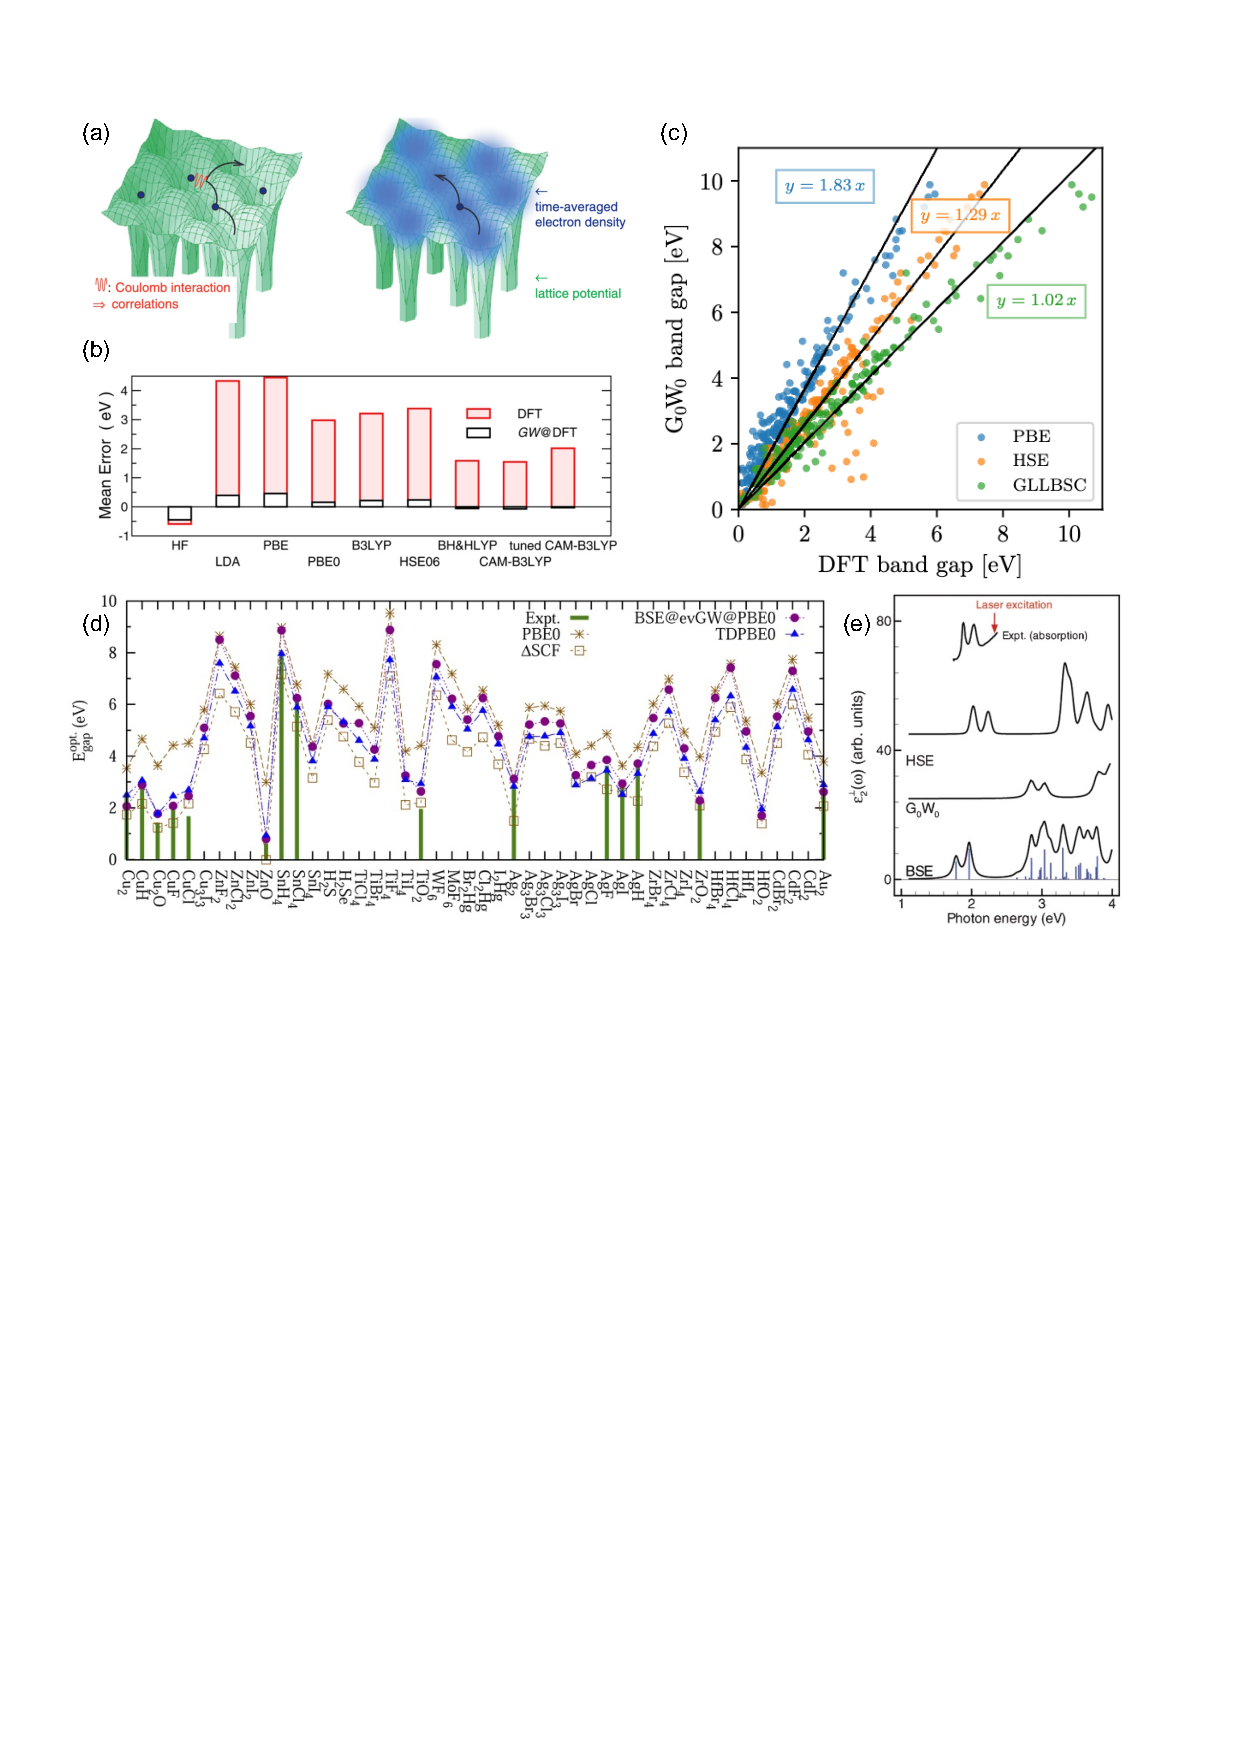
\includegraphics[width=1\linewidth]{GW_approximation_diagram.pdf}
    \caption{(a) In the true many-body system, the electronic correlation is both position- and time-dependent (left), in which the movement of electrons (black curly arrows) are affected by the Coulomb repulsions (red curly line) induced by other neighbouring electrons in the system. On the other hand, mean-field electronic structure theory (such as DFT) simplifies the many-body problem by describing the behaviour of a single electron as moving in a time-averaged potential generated from the other electrons (right) [Adopted from \citet{held2007electronic}]. (b) Deviation of the HOMO energies from the reference CCSD(T) values for a benchmark set of 34 small molecules,\cite{bruneval2013benchmarking} showing the results from different generalised Kohn-Sham (GKS) calculations, that are compared to GW calculations starting from the corresponding GKS orbitals. (c) Band gaps obtained with different DFT functionals plotted against the $G_{0}W_{0}$ results for a database of monolayer 2D materials. The band gaps from PBE (blue), HSE06 (orange), and GLLBSC\cite{kuisma2010kohn} (green) are fitted linearly to the $G_0 W_0$ results. [Adopted from \citet{haastrup2018}]  (d) Optical gaps from PBE0, $\Delta$SCF, the BSE, and TDPBE0, compared to experimental data. [Adopted from \citet{korbel2014benchmark}] (e) Imaginary part of transverse dielectric constant for monolayer \ce{MoS2}, $\varepsilon_{2}^{\perp}(\omega)$, as a function of photon energy $(\hbar\omega)$. Computed spectra are presented for three levels of theory: HSE functional, $G_{0}W_{0}$, and BSE. Vertical (blue) bars represent the relative oscillator strengths for the optical transitions. The two lowest-energy peaks in the spectrum (first two bars) correspond to the A and B excitons. As seen, the closest agreement with experiments in locating the excitionic peaks is obtained at the level of BSE calculations. [Adopted from \citet{ramasubramaniam2012large}]} 
    \label{fig:GW_approximation_diagram}
\end{figure}

Electron correlation arises as the result of the electron-electron Coulomb repulsive potential $\hat{\mathcal{V}}_{ee}$ that enters the many-body Schr\"{o}dinger equation \cref{eq:full_Sch_eqn}. In principle, such effect must be described by the many-body electron wavefunction that varies both in positions and time, \cref{fig:GW_approximation_diagram}(a, left), in which an electron travelling in a material is constantly experiencing and repelled from its original path by the Coulomb repulsions from other surrounding electrons, which are also in constant motions while responding to the Coulomb interactions from each other. This seemingly intractable collective electronic motion is greatly simplified by DFT, which is often referred to as a \textit{mean-field electronic structure theory} because the electron density, the basic variable in DFT, reflects the time-averaged distributions of electrons in the system [\cref{fig:GW_approximation_diagram}(a, right)]. This means that the Kohn-Sham equation effectively describes the behaviour of a single electron in the \textit{mean field} generated by the other electrons in the material. One could imagine this provides a rather crude description on the responses of other electrons.

This problem becomes particularly `magnified' when one considers interpreting the electron spectroscopies.\cite{golze2019gw} In the case of an electron being added to (removed from) a many-body system, the extra electron (hole) will interact with its surrounding electrons, which effectively form a polarisation cloud. This mutual interaction is happening in both ways: the movement of the  extra electron (hole)  is affected by the polarisation cloud, whereas the `shape' of this polarisation cloud will change in response to the Coulomb interaction with the  extra electron (hole)  that is added to the system. Effectively, the true behaviour of this many-body system should be described in terms of \textit{quasiparticle}, which is the extra electron (hole) that is \emph{screened} by its surrounding polarisation cloud. In the many-body theory, the modification to the single-particle energy due to its interaction with the surrounding electrons is given by the \textit{self-energy} $\Sigma$, and the quasiparticle energy is the energy required to remove (add) an electron from HOMO (to LUMO) of the  system, taking into account the electron correlation effect, which corresponds to the ionisation potential (electron affinity) that is measured by the (inverse) photoemission spectroscopy, \emph{i.e}
\begin{equation}
    \label{eq:ionisation_potential}
    \varepsilon_{\mbox{\scriptsize{HOMO}}}=-IP=-[E(N-1)-E(N)],
\end{equation}
and
\begin{equation}
    \label{eq:electron_affinity}
    \varepsilon_{\mbox{\scriptsize{LUMO}}}=-EA=-[E(N)-E(N+1)].
\end{equation}
Here, $E(N)$ represents the (ground-state) energy of a system with $N$ electrons, whereas $E(N+1)$ and $E(N-1)$ represent the (excited-state) energies of the same system with an extra electron added or removed, respectively. However, for DFT that accounts for the electronic correlation effects in a mean-field approach, only \cref{eq:ionisation_potential} holds if the exact exchange-correlation functional is used,\cite{kleinman1997significance} and $\varepsilon_{\mbox{\scriptsize{LUMO}}}\neq-EA$ due to the lack of treatment of the screening effects. This results in the problem such as the underestimation of fundamental gaps in solids and molecules.